\label{chapter:applications}

To demonstrate the impact of GATs, we will present two examples for their applications. The first one was developed in collaboration with one of the involved authors shortly after the original paper was published. Then, a fairly recent publication will highlight the relevance of the architecture to this day.

\section*{GATs for Brain Mesh Segmentation}
In \cite{Cucurull2018ConvolutionalNN}, both GCNs and GATs were cutting edge technologies that were assessed against previous mesh parcellation models. Reconstructions of the cortical surface were represented in a graph which had to be divided into areas. Nodes correspond to locations on the brain surface, their features included cortical thickness, curvature and functional connectivity.

The authors considered three kinds of information the models could use: \textit{neighborhood information}, \textit{node features} and \textit{global information}, that is, access to feature information from all the nodes.
Previous approaches for this task were unable to exploit all three kinds of information and were therefor limited in their complexity. Alongside GCNs, GATs outperformed all state-of-the-art models, showing the importance of utilizing the mesh structure in the data. Furthermore, the authors showed that dynamic attention mechanisms actually improve performance when compared to a constant attention for all neighbors.

\begin{figure}[h]
    \centering
    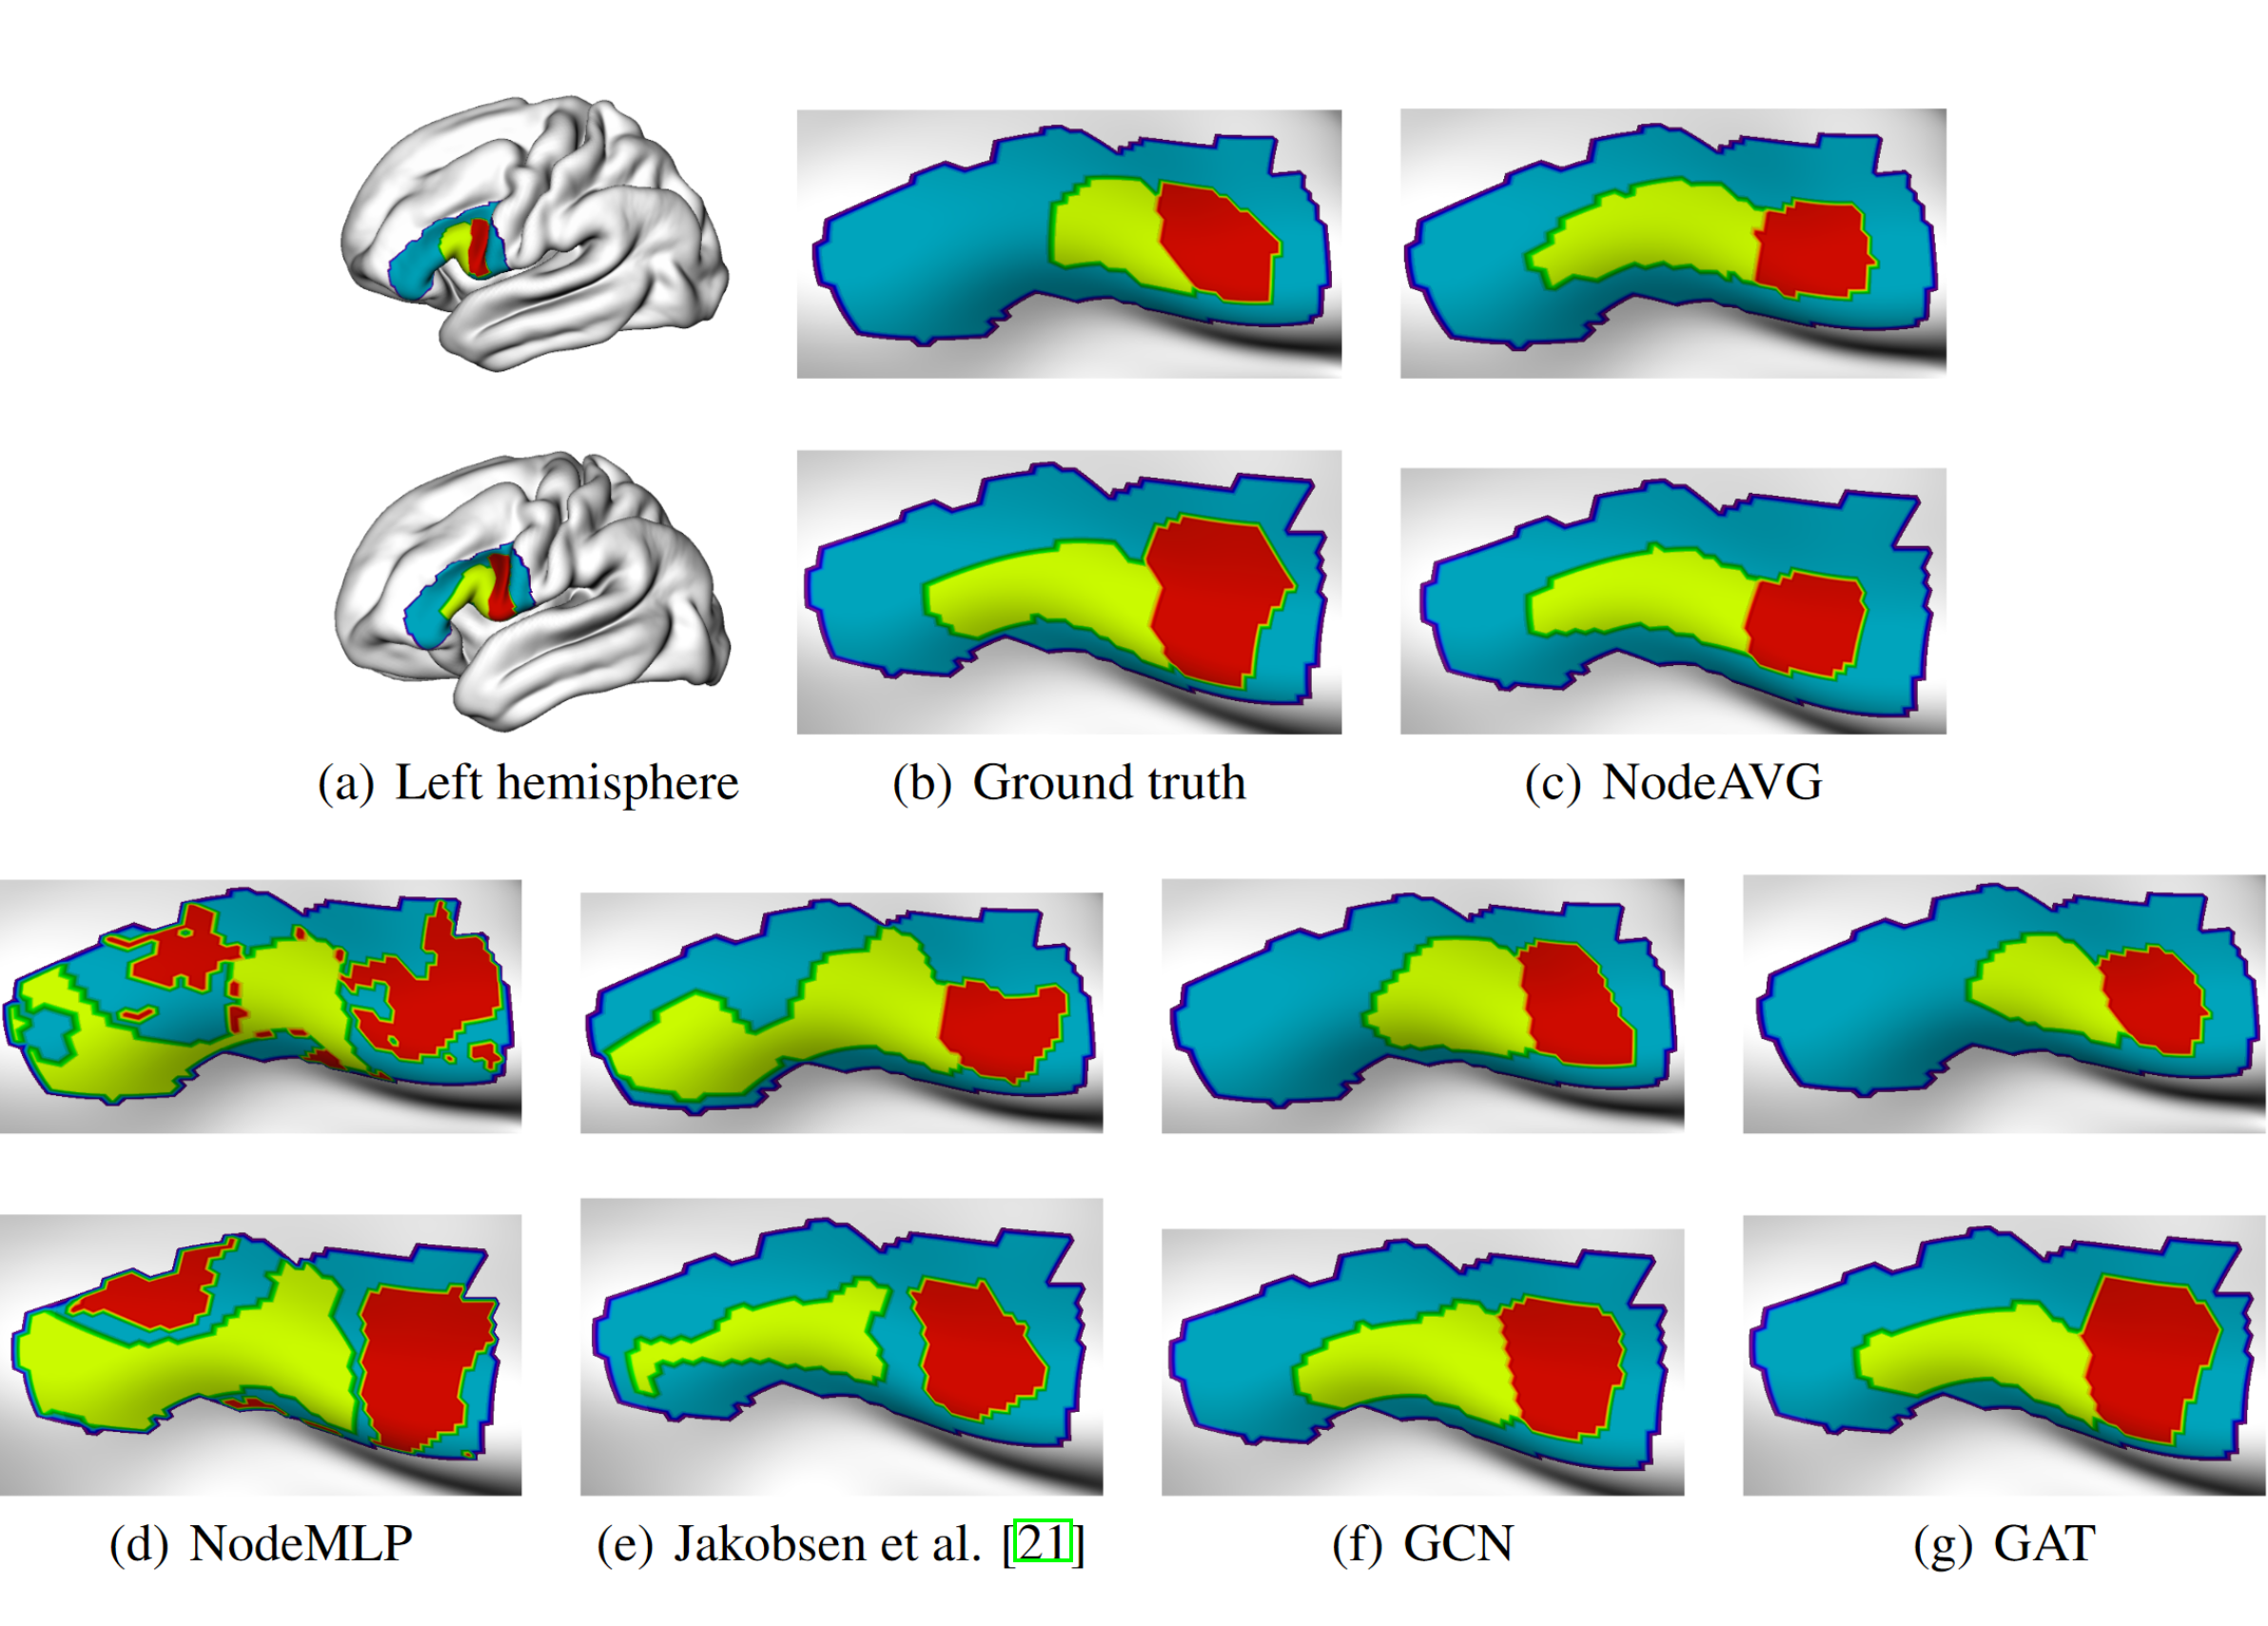
\includegraphics[width=0.75\textwidth]{img/brain_mesh.PNG}
    \caption{Qualitative area parcellation results for two test set subjects. \cite{Cucurull2018ConvolutionalNN}}
\end{figure}

In conclusion, this application demonstrated the potential of GNNs and their applicability to real-world problems. GATs showed promising results, raising hopes for applications in other areas. As we will see later on, this assessment is still up to date and in-line with recent benchmarks.\bigskip

\section*{Improving Explainability through Attention Mechanisms}

Visual Question Answering (VQA) is an important task to build systems that better understand the relationship between vision and language by learning to answer questions about an image. The TextVQA dataset (see \cite{singh2019vqa}) includes image-question pairs that require models to read text in images and answer questions accordingly.

A recent publication by \cite{rao2021look} proposes a model that is able to generate explanations for its answers. These are "consistent with human interpretation, help justify the models' decision and provide useful insights to help diagnose an incorrect prediction". To that end, they build a graph to encode the relatoinship between objects and text. A GAT is then used to variably weigh an object's adjacent text nodes based on relevancy. The attention weights can be visualized as a heat map, highlighting the position of text tokens that were considered important.\medskip

\begin{figure}[h]
    \centering
    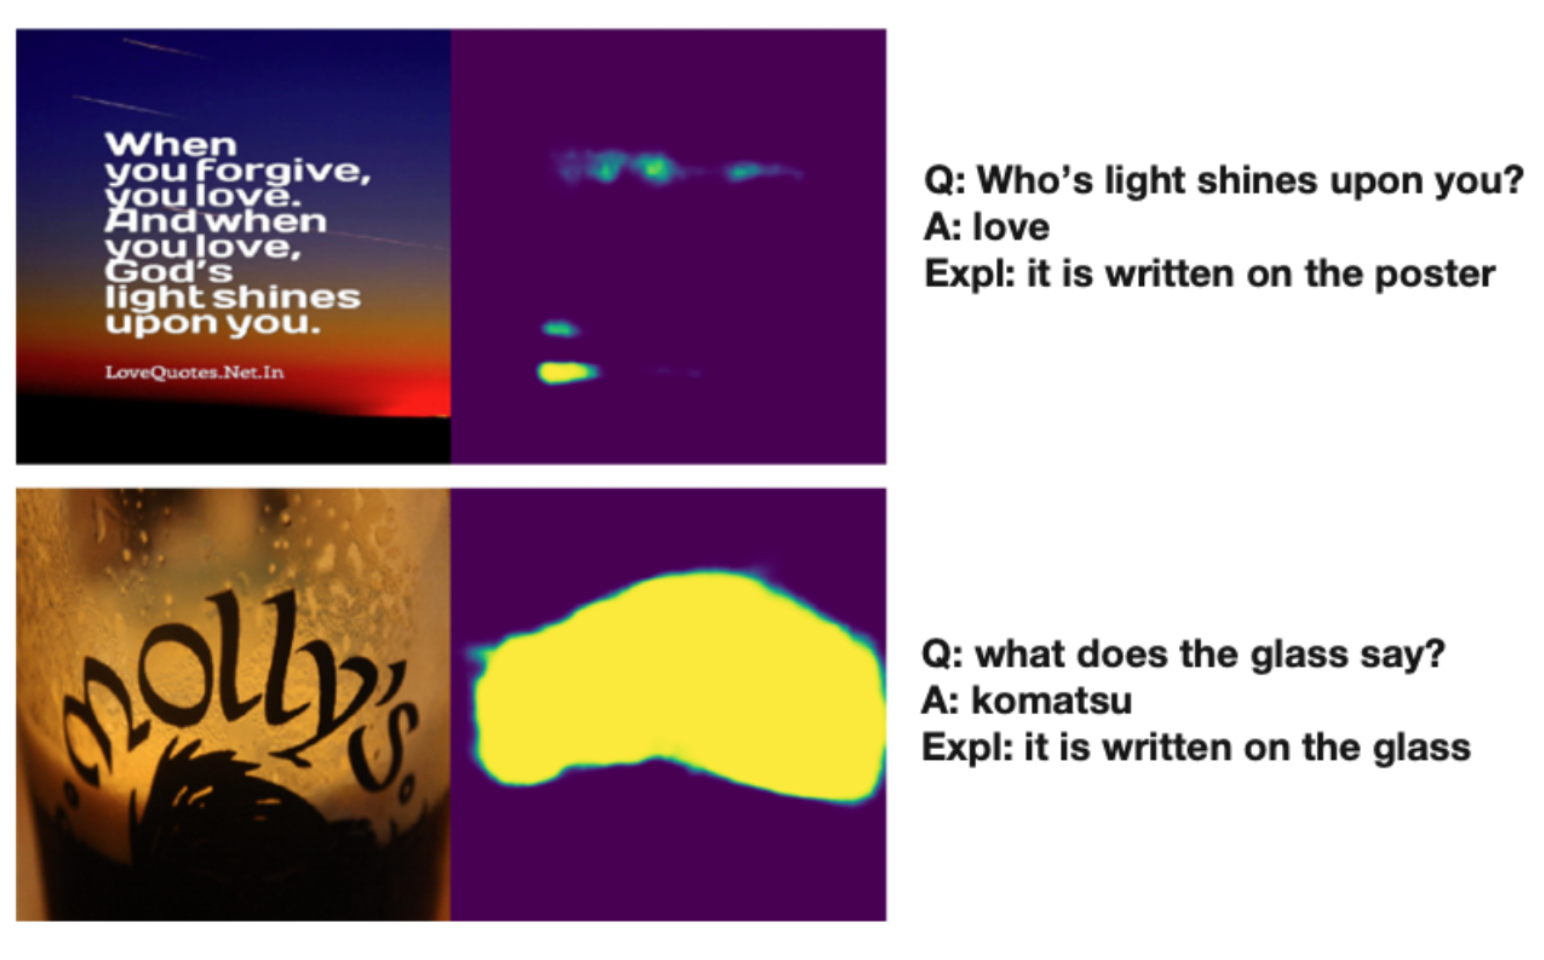
\includegraphics[width=0.75\textwidth]{img/text_3.PNG}
    \caption{Attention weights help explain incorrect decisions. In the first image, the model pays attention to the wrong text tokens. For the second image attention is where it needs to be but the OCR engine fails to read the text correctly. \cite{rao2021look}}
    \medskip
\end{figure}

Allthough there are multiple components to this model, it shows that attention weights can help explain its answers. Therefor, this paper is evidence for the claim about increased interpretability through analysis of attention weights made in \cite{velickovic2018graph}. Once more, it is shown that GATs are still used today and remain an important tool in the graph neural network domain. \bigskip